\chapter{Részletes tervezés}
\label{chap:tervezes}A következő fejezetben részletes betekintés nyújtok, organikus adathalmazzal rendelkező, saját célú hangszerfelismerő rendszer felépítésébe, ismertetve minden tervezési lépést. Ez többek között tartalmazza az adatkészlet létrehozását, a jellemzési paramétereket, az adatbővítési beállításokat és a 2D konvolúciós neurális hálózatokat, a YAMNet transzfer tanulási architektúrát, végül a valós idejű hangszerfelismerő modul tervezését.

%% ═══════════════════════════════════════════════════════════════════════════
\section{Az adathalmaz tervezése}
\label{sec:dataset_design}

Az adathalmaz szigorú szempontrendszer szerint került összeállításra, különös figyelmet szentelve a változatos és felismerhető hangszerjátékra.

Az osztályrendszert hét osztályra osztottuk, amelyek a könnyű és klasszikus zenében előforduló leggyakoribb hangszertípusokat fogják reprezentálni. Van egy extra, környezeti zaj osztály is, amely segítségével kezeljük a csendet és a váratlan hangzavart. A 7 osztály a következő:

\begin{enumerate}
  \item[(1)] Gitár: tartalmazza az akusztikus és a kevésbé torzított elektromos gitárokat is
  \item[(2)] Zongora: tartalmazza a klasszikus és digitális zongorák egyes típusait
  \item[(3)] Vokál: tartalmaz emberi éneklést, rapet és egyéb sajátos hangképzéseket (mongol torokének, szájdob)
  \item[(4)] Húr: a vonós négyes hangszerei: hegedű, brácsa, cselló, bőgő
  \item[(5)] Nádfúvósok: mind egynádas (klarinét, szaxofon), mind kétnádas (fagott, oboa)
  \item[(6)] Rézfúvósok: legelterjedtebb változatok: trombita, harsona, kürt, tuba
  \item[(7)] Zaj: Háttér- és/vagy környezeti zajok (szél, eső, forgalom stb.), madárcsicsergés stb.
\end{enumerate}


\subsection{Saját készítésű organikus adathalmaz}
\label{subsec:own_dataset}

Kezdetben a létező adathalmazokat vizsgáltam, hogy megértsem, hogyan érdemes elkezdeni a tervezési folyamatot, és megfigyeljem, miben erősek külön-külön. Ennek érdekében az előkészítő szakaszban lefuttattam egy elemző szkriptet (\texttt{01\_analyze\_\allowbreak datasets.py}), amely feltárta az elérhető források struktúráját. Az elemzés eredményeit a \ref{tab:adathalmaz_osszehasonlitas}.~táblázat foglalja össze.

\begin{table}[H]
\centering
\caption{A vizsgált publikus adathalmazok összehasonlító elemzése}
\label{tab:adathalmaz_osszehasonlitas}
\begin{tabular}{p{2.2cm}p{4.0cm}p{4.0cm}p{3.6cm}}
\toprule
\textbf{Adathalmaz} & \textbf{Tartalom leírása} & \textbf{Fő erősségek} & \textbf{Korlátok / Miért nem felelt meg} \\
\midrule
\textbf{IRMAS}~\cite{bosch2012irmas} & Zenei részletek (3~s) szóló hangszeres és polifón szekciókkal & Valós zenei környezet, polifónia vizsgálata & Korlátozott számú és egyenetlen eloszlású hangszerkategóriák. \\
\addlinespace
\textbf{NSynth}~\cite{engel2017nsynth} & 300\,000+ db egyedi hangszeres hangjegy (4~s) & Hatalmas mintaállomány, egységes hanghossz és pitch & Csak izolált hangok, nincs benne valós zenei folytonosság és frazeálás. \\
\addlinespace
\textbf{Medley-solos-DB}~\cite{lostanlen2018medley} & Különböző sávokból kinyert szóló hangszeres részek (3~s) & Valós zenei előadásokból származó, tiszta szóló felvételek & Alacsony mintaszám egyes kategóriákban, szűkös osztályválaszték. \\
\addlinespace
\textbf{TinySOL}~\cite{cella2020tinysol} & Izolált zenekari hangszerek hangjai, különböző technikákkal & Kiváló stúdióakusztika, gazdag játéktechnikai annotációk & Kizárólag izolált hangjegyek, nem reprezentálja a folyamatos zenélést. \\
\addlinespace
\textbf{Good-sounds}~\cite{romani2015good} & Fúvós és vonós hangszerek egyedi hangjegyei & Különböző minőségű mikrofonok és felvételi minőségek & Nagyon szűk hangszerpaletta (pl. nincs gitár vagy énekhang). \\
\addlinespace
\textbf{ESC-50}~\cite{piczak2015esc} & 2000 db környezeti és háttérzaj minta (5~s) & 50 különböző zajkategória rendkívül széles spektruma & Nem tartalmaz zenei hangszereket, csak a zaj kategóriához alkalmas. \\
\bottomrule
\end{tabular}
\end{table}

Megállapítottam, hogy a meglévő adathalmazok teljes vagy részleges felhasználása nem felel meg az igényeimnek. Minden adathalmaz mintái eltérő hosszúságúak, más a hangszerosztályok eloszlása, rengeteg mintát tartalmaznak, és különböző céllal jöttek létre. Emiatt – bár kiváló tervezési alapul szolgáltak – a feldolgozásuk egységesítése komplex feladat lenne, és az átválogatásuk is rengeteg időt igényelne. Egy organikus, a saját elképzeléseim alapján összeállított adathalmaz biztosabb és átláthatóbb alapokat nyújt egy jól működő modell megteremtéséhez. 
Ez alól kivételt képezett az ESC-50, amely sokféle környezeti és háttérzaj-mintát foglal magába, így hiánypótlóként szolgált egy mindenre kiterjedő zajos adathalmaz összeállításához.

Az interneten található zenei felvételekből válogattam, figyelmet fordítva az aktuális hangszerek karakterességének kiemelésére és a zenei játék változatosságára. Minden hangszerosztályhoz (gitár, zongora, ének, vonós, nád- és rézfúvós) nagyjából 100--150 darab interneten elérhető felvételt választottam ki, amelyekből az eredeti forrás zenei tartalmának függvényében 5 másodperces blokkokat vágtam ki. 

Ezen a ponton egy kritikus tervezési döntést hoztam a gépi tanulásban gyakran felmerülő adatszivárgás (data leakage) elkerülése érdekében. Ha a darabolást rögtön végrehajtom, majd az összes 1 másodperces szeletet utólag osztom szét, nagy az esélye annak, hogy ugyanannak a hangszernek ugyanabból a zenei frázisából kerüljenek minták mind a tanító (train), mind a validációs (val) vagy teszt (test) halmazba. Ez túlzottan optimista, hamis eredménybecsléshez (túltanuláshoz, azaz overfittinghez) vezetne, mivel a modell szinte azonos hangokat látna a teszteléskor, mint a tanításkor.

Ennek elkerülésére a \texttt{01\_prepare\_clean\_dataset.py} szkript segítségével először a teljes, 5 másodperces blokkokat kevertem meg és osztottam fel a tanító (70\%), validációs (15\%) és tesztelő (15\%) halmazokra. Ezt a műveletet úgynevezett \textbf{rétegzett (stratified) felosztással} végeztem el, ami garantálja, hogy a szkript minden egyes hangszerosztálynál önállóan és szigorúan betartsa ezt az arányt, így az osztályok eloszlása mindhárom halmazban (train, val, test) tökéletesen megegyező és kiegyensúlyozott marad. A szkript csak ezután – a már szigorúan szeparált blokkokat – szeletelte fel 1 másodperces, átfedésmentes klipekre, megőrizve a szeparáció integritását. Ezáltal biztosítható, hogy a kiértékelési halmazok (val/test) eredményei teljesen megbízhatóak, és a modell nem tud ,,csalni''.

Ez a folyamat hangszertípusonként nagyjából 500 darab, többnyire monofón, stúdió- és szobaminőségű mintát eredményezett. A teljes tiszta adathalmaz (beleértve az ESC-50-ből származó kiterjedt zaj osztályt is) így összesen 4428 mintából áll.

Fontosnak tartom hangsúlyozni, hogy az internetről gyűjtött zenei hangmintákat kizárólag kutatási és oktatási (akadémiai) célokra használom fel. Ezeket a mintákat önmagukban nem teszem közzé, nem terjesztem nyilvánosan, és semmilyen kereskedelmi vagy pénzszerzési célra sem használom fel. Ez a megközelítés teljesen analóg a nagy technológiai vállalatok által alkalmazott gyakorlattal, ahol a nyilvánosan elérhető adatokat szigorúan a modellek tanítására használják fel (a szabad felhasználás, azaz a \textit{fair use} elve alapján), miközben maguk a nyers forrásfájlok zártak maradnak.

Az adathalmaz eloszlását ezen lépés után a \ref{fig:organic_class_distribution}.~ábra szemlélteti.

\begin{figure}[H]
\centering
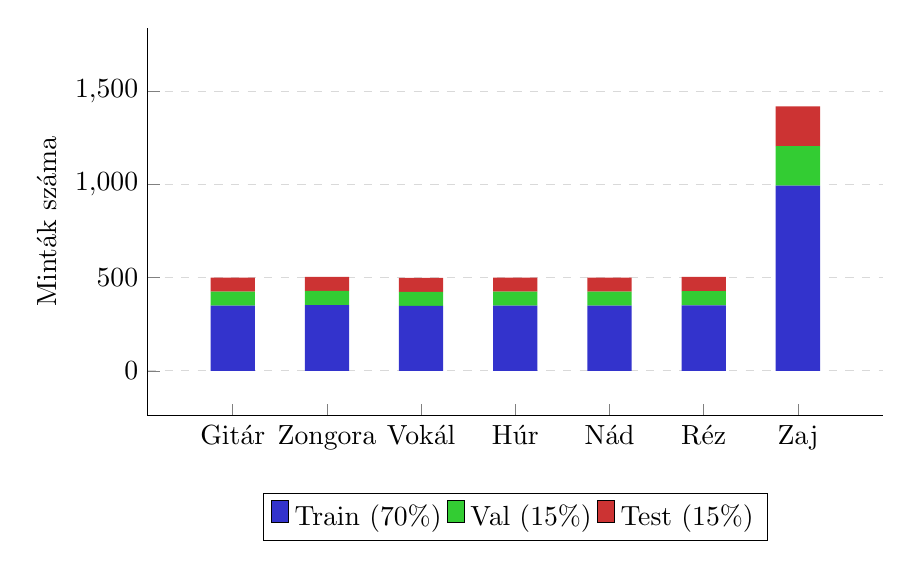
\begin{tikzpicture}
\begin{axis}[
    ybar stacked,
    bar width=16pt,
    enlargelimits=0.15,
    ylabel={Minták száma},
    symbolic x coords={Gitár, Zongora, Vokál, Húr, Nád, Réz, Zaj},
    xtick=data,
    ymin=0,
    ymax=1600,
    width=0.9\textwidth,
    height=6.5cm,
    axis x line*=bottom,
    axis y line*=left,
    ymajorgrids=true,
    grid style={dashed, gray!30},
    legend style={at={(0.5,-0.2)}, anchor=north, legend columns=-1},
]
\addplot[fill=blue!60!gray, draw=none] coordinates {
    (Gitár,350) (Zongora,353) (Vokál,349) (Húr,350) (Nád,350) (Réz,352) (Zaj,994)
};
\addplot[fill=green!60!gray, draw=none] coordinates {
    (Gitár,75) (Zongora,76) (Vokál,75) (Húr,75) (Nád,75) (Réz,76) (Zaj,213)
};
\addplot[fill=red!60!gray, draw=none] coordinates {
    (Gitár,75) (Zongora,76) (Vokál,75) (Húr,75) (Nád,75) (Réz,76) (Zaj,213)
};
\legend{Train (70\%), Val (15\%), Test (15\%)}
\end{axis}
\end{tikzpicture}
\caption{A saját gyűjtésű organikus adathalmaz eloszlása a szeparált szeletelés után}
\label{fig:organic_class_distribution}
\end{figure}

\subsection{Mikrofonos újrafelvétel a valós idejű kiértékelés felkészítésének érdekében}
\label{subsec:mic_recording}

A kezdeti adatkészleteim önmagukban kevés zajos mintát tartalmaznak, melyeket az eredeti felvételt készítő eszköz mikrofonjával rögzítettek. Minden mikrofonnak saját jellemzői vannak: frekvencia-válasza, érzékenysége, torzítása, belső zaja és maximális hangnyomásszintje (SPL). Mivel a projektem célja a valós idejű hangszerfelismerés is, a modell stabilitásának kialakításához elengedhetetlen az optimalizálás a saját eszközünkre, amellyel a predikció megtörténik.

A valós idejű kiértékelésre való felkészítés érdekében egy speciális eljárást találtam ki. Mivel nem férek hozzá, és játszani sem tudok ennyiféle hangszeren, a telefon hangszóróján játszom vissza a mintákat a laptopom beépített mikrofonjába. A feljátszás 10--30~cm távolságról történik a beépített mikrofon pontos helyzetétől mérve, hogy a hang a közelség miatt se legyen túl torz, de a távolság miatt se váljon értelmezhetetlenné vagy túl halkká.

A több ezer minta egyenkénti feljátszása helyett egy automatizált munkafolyamatot alakítottam ki. Egyetlen közös script (\texttt{02\_acquire\_\allowbreak mic\_\allowbreak data.py}) segítségével először osztályonként összefűzöm a tiszta adatok 70\%-át kitevő tanító (train) halmaz mintáit, a telefonról visszajátszva egyben felvételezem, majd a szoftver automatikusan újra felszeleteli azokat. Ezt követően egy dedikált script (\texttt{03a\_merge\_\allowbreak mic\_\allowbreak to\_\allowbreak train.py}) végzi el az új mikrofonos minták célirányos fúzióját a tanító adathalmazzal. Kritikus tervezési döntés, hogy ezt a mikrofonos újrafelvételt kizárólag a tanító halmazon végzem el, míg a validációs és teszt halmazok teljesen ,,tiszták'' maradnak. Ezzel elkerülhető az adatszivárgás (data leakage): ha a modell a tesztelés során a saját mikrofonunk már megismert alapzajával és torzításával találkozna, a specifikus zajokat felismerve ,,csalhatna''. A tiszta kiértékelő halmazok garantálják, hogy a modell valós generalizációs képességét mérjük egy számára teljesen ismeretlen akusztikai környezetben.

Ebben az esetben azonban a telefon lejátszásának és a laptop beépített mikrofonjának felvételezésének szinkronizációjára van szükség. A pontos szinkronizáció megvalósításához a következő folyamatot alakítottam ki: a \texttt{02\_acquire\_\allowbreak mic\_\allowbreak data.py} script első előkészítő lépése a hanganyag legelejére egy 1~másodperces, 440~Hz-es szinuszos szinkronizációs sípszót generál, a hangszeres mintákat pedig 0,2~másodperces csendes szakaszokkal választja el egymástól. A telefonról történő visszajátszás alatt ugyanez a script rögzíti a beérkező jelet 16\,000~Hz-es mintavételezéssel, mono formátumban. Végül a script szeletelő funkciója a Librosa könyvtár segítségével detektálja a felvétel elején található sípszó végét, majd ettől a ponttól kiindulva felszeleteli a hanganyagot pontosan 1~másodperces egységekre, miközben automatikusan kiszűri a csendes részeket.
 
Az automatizált mikrofonos újrafelvételi és szeletelési munkafolyamatot a \ref{fig:mic_recording_pipeline}.~ábra szemlélteti.

\begin{figure}[H]
\centering
\begin{tikzpicture}[
    node distance=1.2cm and 0.8cm,
    block/.style={draw, rectangle, minimum height=1.5cm, minimum width=2.4cm, fill=blue!5!white, text width=2.2cm, align=center, font=\footnotesize, rounded corners},
    arrow/.style={thick,->,>=stealth}
]
% Nodes
\node (orig) [block] {Tiszta train minták (70\%)};
\node (concat) [block, right=0.8cm of orig] {Összefűzés (szinkronizációs sípszóval)};
\node (play) [block, right=0.8cm of concat] {Lejátszás (Telefon)};
\node (record) [block, below=1.2cm of play] {Laptop rögzítés (Beépített mikrofon)};
\node (sync) [block, left=0.8cm of record] {Szinkronizáció (sípszó detektálás)};
\node (slice) [block, left=0.8cm of sync] {Szeletelés és beolvasztás (Train)};

% Arrows
\draw [arrow] (orig) -- (concat);
\draw [arrow] (concat) -- (play);
\draw [arrow] (play) -- (record);
\draw [arrow] (record) -- (sync);
\draw [arrow] (sync) -- (slice);

\end{tikzpicture}
\caption{A mikrofonos újrafelvételi és szinkronizált szeletelési folyamat lépései}
\label{fig:mic_recording_pipeline}
\end{figure}

Az újrafelvételi folyamat eredményeképpen kizárólag a tanító (train) halmaz eredeti, tiszta mintái mellé kerülnek be az új, mikrofonos karakterisztikájú minták. Ez a bővítmény hordozza a laptopom beépített mikrofonjának torzításait, frekvencia-válaszát és belső zaját, felkészítve ezzel a modellt a valós idejű kiértékelés kihívásaira. Az adathalmaz aktuális összetételét és a minták felhalmozódását a \ref{fig:mic_recorded_distribution}.~ábra szemlélteti egymásra épülő (stacked) formában, halmazok (Train, Val, Test) és rögzítési mód (Tiszta, Mikrofonos) szerint különválasztva. Fontos megjegyezni, hogy a Zaj osztály esetében nem végeztem ilyen újrafelvételt: az ebből a kategóriából származó ESC-50 minták eleve valós környezeti és háttérzajokat tartalmaznak, így teljesen feleslegesnek tartottam a szélzaj vagy az eső hangját telefonról visszajátszva újra felvenni, ráadásul ez a lejátszási lánc miatt szükségtelen egyedi torzulásokat is vinne a tiszta zajmintákba.

\begin{figure}[H]
\centering
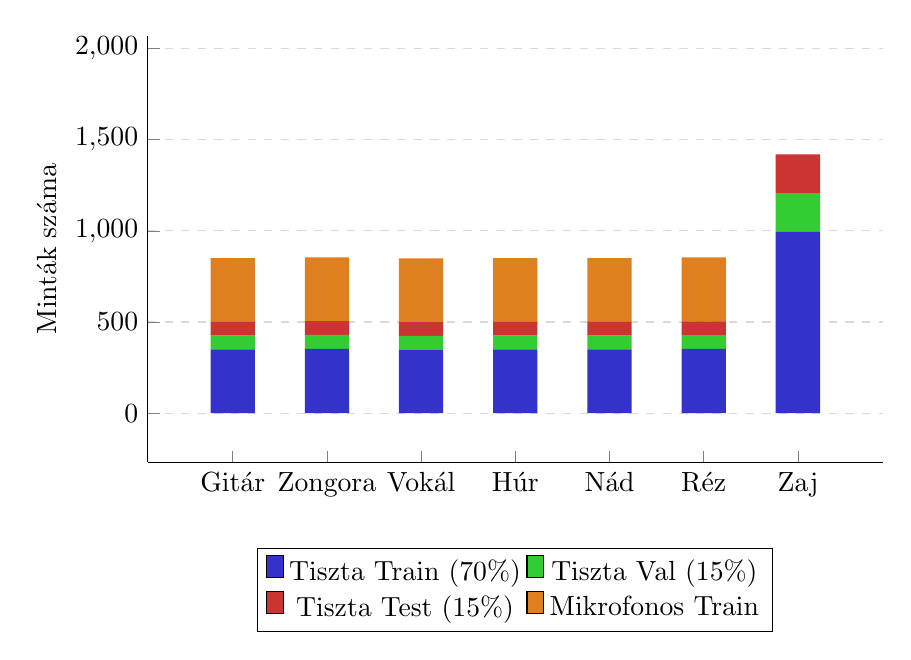
\begin{tikzpicture}
\begin{axis}[
    ybar stacked,
    bar width=16pt,
    enlargelimits=0.15,
    ylabel={Minták száma},
    symbolic x coords={Gitár, Zongora, Vokál, Húr, Nád, Réz, Zaj},
    xtick=data,
    ymin=0,
    ymax=1800,
    width=0.9\textwidth,
    height=7cm,
    axis x line*=bottom,
    axis y line*=left,
    ymajorgrids=true,
    grid style={dashed, gray!30},
    legend style={at={(0.5,-0.2)}, anchor=north, legend columns=2},
]
\addplot[fill=blue!60!gray, draw=none] coordinates {
    (Gitár,350) (Zongora,353) (Vokál,349) (Húr,350) (Nád,350) (Réz,352) (Zaj,994)
};
\addplot[fill=green!60!gray, draw=none] coordinates {
    (Gitár,75) (Zongora,76) (Vokál,75) (Húr,75) (Nád,75) (Réz,76) (Zaj,213)
};
\addplot[fill=red!60!gray, draw=none] coordinates {
    (Gitár,75) (Zongora,76) (Vokál,75) (Húr,75) (Nád,75) (Réz,76) (Zaj,213)
};
\addplot[fill=orange!75!gray, draw=none] coordinates {
    (Gitár,350) (Zongora,350) (Vokál,350) (Húr,350) (Nád,350) (Réz,350) (Zaj,0)
};
\legend{Tiszta Train (70\%), Tiszta Val (15\%), Tiszta Test (15\%), Mikrofonos Train}
\end{axis}
\end{tikzpicture}
\caption{A saját tiszta és az újrafelvételezett zajos minták megoszlása az adathalmazban}
\label{fig:mic_recorded_distribution}
\end{figure}

\subsection{Végső adathalmaz összeállítása}
\label{subsec:final_dataset}



Egy konzisztens és pontos adathalmaz nagyban segíti a neurális hálózat tanulási folyamatát. A megtervezett adatfolyam két fő könyvtárra támaszkodik: a \texttt{dataset\_clean} (amely a tiszta internetes mintákat tartalmazza, összesen 4428 darabot) és a \texttt{dataset\_mic} (amely a \texttt{train} halmaz esetében már tartalmazza az újrafelvett, mikrofonos mintákat is, így összesen 6492 darabot számol).

Amikor a jellemzőkinyerő script lefut, az adataugmentációs lépéseket (reverb, zajkeverés, torzítás) ,,on-the-fly'', azaz dinamikusan végzi el a memóriában. Ennek eredményeképpen a feldolgozott (kinyert) jellemzők száma a tanítási fázishoz kibővül: a tiszta adathalmazban 5927-re, míg a mikrofonos (augmented) adathalmazban 8335-re. Ez a megközelítés rendkívül stabil alapokat biztosít a hálózat számára.

\section{Jellemzőkinyerés tervezése}
\label{sec:feature_extraction}

A nyers audiojelek nem alkalmasak közvetlenül a konvolúciós neurális hálózat bemeneteként, mivel a hullámforma (waveform) időtartománybeli ábrázolása túl magas dimenziójú és nehezen tanulható mintázatokat tartalmaz. Emiatt szükséges egy megfelelő 2D-s spektrális jellemzőkinyerési eljárás kiválasztása. A tervezés során három elterjedt módszert vizsgáltam meg a \texttt{librosa}~\cite{mcfee2015librosa} könyvtár implementációira építve: a rövid idejű Fourier-transzformációt (STFT), a Mel-frekvenciás kepsztrális együtthatókat (MFCC), valamint a Log-Mel spektrogramot. Mindhárom jellemzőtípus azonos ablakozási paraméterekkel készül:

\begin{itemize}
  \item FFT ablakméret: $n\_fft = 1024$ minta,
  \item Ugrási hossz (hop length): $hop\_length = 512$ minta,
  \item Mintavételi frekvencia: $SR = 16\,000$ Hz.
\end{itemize}

1~másodperces audioszelet esetén ($16\,000$ minta, $hop\_length = 512$) az időtengely mérete: $\lfloor 16000 / 512 \rfloor + 1 = 32$ időkeret.

\subsection{Log-Mel spektrogram}

A Log-Mel spektrogram előállításának lépései:

\begin{enumerate}
  \item Mel-szűrőbank alkalmazása $n\_mels = 64$ sávval az STFT kimenetére,
  \item Teljesítmény-decibelre konvertálás: $S_{dB} = 10 \cdot \log_{10}(S_{mel} / S_{ref})$.
\end{enumerate}

Az eredmény egy $64 \times 32$ méretű mátrix, amelyet a CNN egycsatornás képként ($64 \times 32 \times 1$) kap meg. A Log-Mel spektrogram előnye, hogy a Mel-skála a hallórendszer nemlineáris frekvenciaérzékelését modellezi, így a hangszerek jellegzetes formánsai és felharmonikusai hatékonyan jelennek meg.

\subsection{STFT spektrogram}

Az STFT (Short-Time Fourier Transform) spektrogram az amplitúdó-spektrum decibelre konvertált változata:

$$X_{dB}(f,t) = 20 \cdot \log_{10}\left(\frac{|X(f,t)|}{X_{ref}}\right)$$

Az eredmény egy $513 \times 32$ méretű mátrix ($n\_fft/2 + 1 = 513$ frekvenciasáv). Ez a reprezentáció a teljes lineáris frekvenciaskálát megtartja.

\subsection{MFCC (Mel-Frequency Cepstral Coefficients)}

Az MFCC-t $n\_mfcc = 40$ együtthatóval számolom. Az MFCC a spektrális burkoló tömör reprezentációja; az eredmény egy $40 \times 32$ méretű mátrix. Az MFCC jellemzőkre Z-score normalizálást alkalmazok sávonként:

$$\hat{x}_i = \frac{x_i - \mu_i}{\sigma_i + \epsilon}$$

ahol $\mu_i$ és $\sigma_i$ az $i$-edik MFCC sáv átlaga és szórása, $\epsilon = 10^{-10}$.

\subsection{Nyers hanghullám (Raw waveform)}

A frekvenciatartománybeli jellemzők mellett közvetlenül kinyerjük és elmentjük a nyers, időtartománybeli audiojelet is. 1 másodperc esetén ez egy 16\,000 elemű, 1D-s tömb. Bár a hagyományos 2D CNN hálózatok számára ez az ábrázolás nem ideális, a mélyebb transzfer tanulási eljárások (például a YAMNet) pontosan ezt a nyers formátumot várják bemenetként.

\subsection{A megfelelő jellemzőkinyerési eljárás kiválasztása}
\label{subsec:feature_selection}

A három vizsgált jellemzőtípus (STFT, MFCC, Log-Mel) alapos elemzése után a következő szempontokat mérlegeltem a neurális hálózat bemenetének kiválasztásakor:
\begin{itemize}
  \item Az \textbf{STFT spektrogram} előnye, hogy a teljes lineáris frekvenciaspektrumot megőrzi, azonban a $513 \times 32$-es méret túl nagy dimenziójú bemenetet eredményezne. Ez nemcsak jelentősen növelné a hálózat paraméterszámát és a tanítási időt, de a magas frekvenciás sávok felesleges részletgazdagsága miatt a túlilleszkedés (overfitting) kockázatát is növelné.
  \item Az \textbf{MFCC} bár rendkívül kompakt ($40 \times 32$), a diszkrét koszinusz transzformáció (DCT) alkalmazásával eldobja a spektrális finomszerkezetet és a felharmonikusok közötti összefüggéseket. Ez beszédfelismerésnél előnyös (ahol a hangmagasságtól független fonémákat keressük), de a zenei hangszerek osztályozásánál a felharmonikusok aránya hordozza a hangszín lényegi információját, így az MFCC használata információvesztéssel járna.
  \item A \textbf{Log-Mel spektrogram} ($64 \times 32$) jelenti a legjobb kompromisszumot. A Mel-skála nemlineárisan sűríti a frekvenciatengelyt az emberi hallásnak megfelelően (finomabb felbontás a mély tartományban, durvább a magasban), így megőrzi a hangszerek hangszínének felismeréséhez szükséges felharmonikus-szerkezetet, miközben alacsonyan tartja a bemeneti dimenziót.
\end{itemize}

A fenti szempontok alapján a valós idejű hangszerfelismerő rendszerem elsődleges jellemzőjének a \textbf{Log-Mel spektrogramot} választottam, a konvolúciós neurális hálózat architektúráját és a valós idejű feldolgozást is erre a bemenetre terveztem. A három vizsgált jellemző legfontosabb tulajdonságait a~\ref{tab:feature_comparison_properties}. táblázat foglalja össze.

\begin{table}[H]
  \centering
  \caption{A három vizsgált jellemzőkinyerési módszer összehasonlító elemzése}
  \label{tab:feature_comparison_properties}
  \resizebox{\textwidth}{!}{%
  \begin{tabular}{lllp{4.5cm}p{4.5cm}}
    \toprule
    \textbf{Jellemző} & \textbf{Dimenzió} & \textbf{Frekvencia-skála} & \textbf{Fő előny} & \textbf{Fő hátrány} \\
    \midrule
    STFT & $513 \times 32$ & Lineáris & Megőrzi a teljes spektrális finomszerkezetet. & Túl nagy dimenziószám, növeli a túlilleszkedés kockázatát. \\
    \midrule
    Log-Mel & $64 \times 32$ & Logaritmikus Mel-skála & Az emberi hallást modellezi; megőrzi a felharmonikusokat. & Enyhe információvesztés a frekvenciatömörítés miatt. \\
    \midrule
    MFCC & $40 \times 32$ & Kepsztrális & Rendkívül kompakt és dekorrelált reprezentáció. & Diszkrét koszinusz transzformáció miatt eldobja a felharmonikusokat. \\
    \bottomrule
  \end{tabular}%
  }
\end{table}

\subsection{Normalizálás}

A kiválasztott Log-Mel jellemzőket globális min-max normalizálással skálázom a $[0, 1]$ intervallumra:

$$\hat{X} = \frac{X - X_{min}}{X_{max} - X_{min} + \epsilon}$$

Ez biztosítja, hogy a CNN bemenete konzisztens értéktartományban maradjon.

\begin{figure}[H]
  \centering
  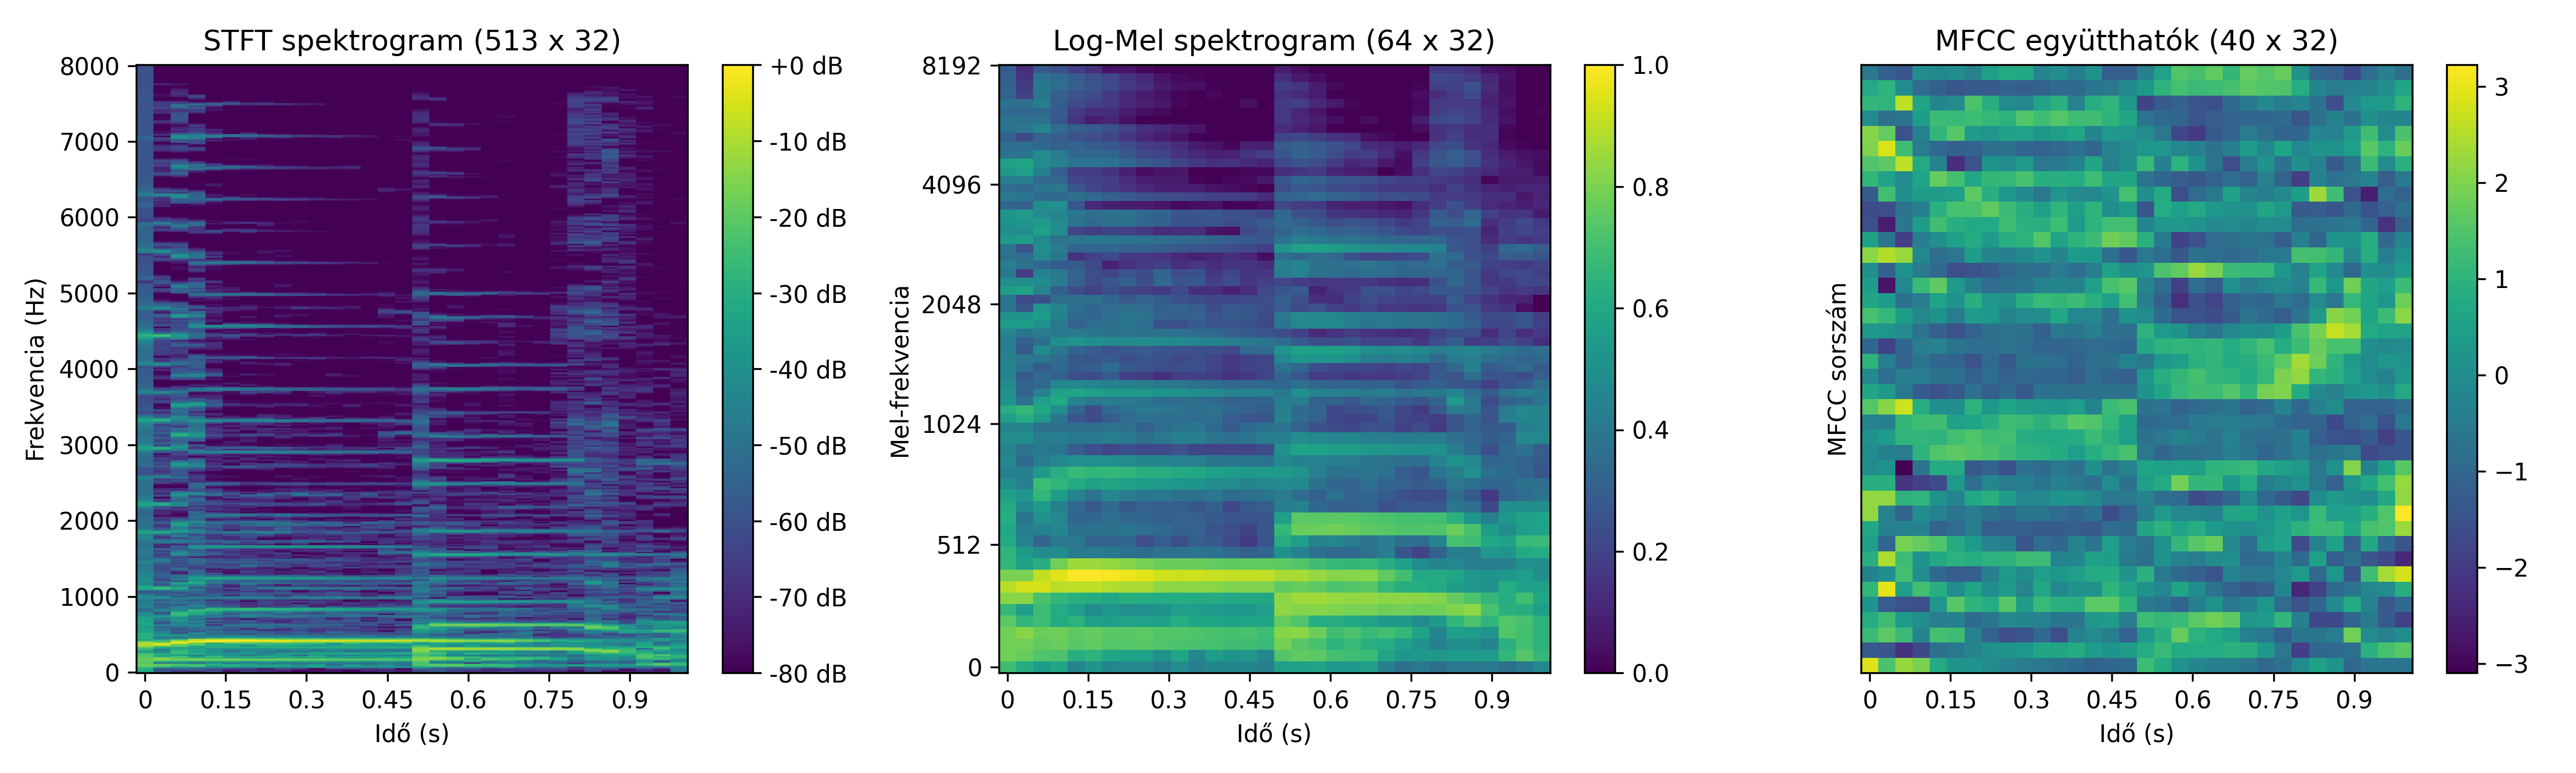
\includegraphics[width=\textwidth]{fig_feature_comparison.png}
  \caption{A három vizsgált jellemzőtípus vizualizációja ugyanazon gitárminta esetén: (a) STFT spektrogram ($513 \times 32$), (b) normalizált Log-Mel spektrogram ($64 \times 32$), (c) normalizált MFCC együtthatók ($40 \times 32$)}
  \label{fig:feature_comparison}
\end{figure}

\subsection{Jellemzőkinyerés kimeneti állományai}
\label{subsec:feature_outputs}

A jellemzőkinyerési folyamat sikeres lefutása után a kinyert mátrixok és a hozzájuk tartozó osztálycímkék a projekt gyökerében lévő \texttt{processed\_data\_clean/} és \texttt{processed\_data\_mic/} könyvtárakba kerülnek elmentésre NumPy formátumban (\texttt{.npy} kiterjesztéssel), az alkalmazott forrásadathalmaztól függően. A generált fájlok már nem egyetlen nagy tömbben, hanem a szeparált kiértékelési halmazoknak megfelelően szétbontva (\texttt{train}, \texttt{val}, \texttt{test}) készülnek el. Például a \texttt{train} halmazhoz tartozó fájlok a következők:
\begin{itemize}
  \item \textbf{Log-Mel spektrogram:} \texttt{X\_log\_mel\_train.npy} (a jellemzőmátrixokat tartalmazó tömb) és \texttt{y\_labels\_train.npy} (a hangszerosztályok sorszámait tartalmazó címketömb),
  \item \textbf{STFT spektrogram:} \texttt{X\_stft\_train.npy},
  \item \textbf{MFCC együtthatók:} \texttt{X\_mfcc\_train.npy},
  \item \textbf{Nyers hanghullám (csak a mic adathalmaznál):} \texttt{X\_raw\_train.npy}, amely az olyan transzfer tanulási architektúrák, mint a YAMNet, közvetlen bemeneteként szolgál.
\end{itemize}
A normalizált és binárisan tömörített fájlformátum biztosítja, hogy a tanítási fázisban a minták betöltése rendkívül gyorsan, közvetlenül a memóriába (RAM) történhessen meg, elkerülve a felesleges lemezműveleteket.

%% ═══════════════════════════════════════════════════════════════════════════
\section{Adataugmentáció tervezése}
\label{sec:augmentation}

A modell valós idejű kiértékelésre való felkészítése érdekében a tanító (train) halmaz minden tiszta hangszermintáját (a noise osztályt és az eleve mikrofonnal rögzített \texttt{\_mic\_} mintákat kivéve) egy augmentált változattal egészítek ki. Az augmentáció a fogyasztói mikrofonos felvétel körülményeit szimulálja, ezért a belső elnevezése \texttt{apply\_macbook\_\allowbreak augment}. Az alkalmazott adataugmentációs lánc felépítését és a lépések sorrendjét a \ref{fig:augmentation_chain}.~ábrán mutatom be, míg az augmentáció hatását a spektrális jellemzőkre (egy gitárminta példáján keresztül) a \ref{fig:original_vs_augmented}.~ábra szemlélteti.

Az augmentációs lánc a következő lépésekből áll:

\subsection{Szobai reverb szimuláció}
\label{subsec:reverb}

A reverb szimulációt 80\%-os valószínűséggel alkalmazom. A szoba akusztikáját egy egyszerű FIR visszhang-modellel közelítem, amely négy visszaverődési pontot (tap) használ:

\begin{itemize}
  \item Késleltetés (\textit{delay}): véletlenszerű, 15--40 ms között,
  \item Csillapítási tényező (\textit{decay}): véletlenszerű, 0{,}2--0{,}45 között,
  \item Visszaverődési pontok: $d$, $1{,}5d$, $2{,}1d$, $2{,}8d$ mintányi késleltetésnél,
  \item Csillapítás: $decay^1$, $decay^2$, $decay^3$, $decay^4$.
\end{itemize}

\subsection{Frekvenciaválasz-torzítás (Pre-emphasis)}

A mikrofon és a szoba együttes frekvenciaválaszának szimulálására pre-emphasis szűrőt alkalmazok, amelynek együtthatója véletlenszerűen 0{,}92 és 0{,}98 között változik:

$$y[n] = x[n] - \alpha \cdot x[n-1]$$

\subsection{Környezeti zajkeverés (Noise mixing)}

A háttérzajt az ESC-50 adathalmaz~\cite{piczak2015esc} véletlenszerűen kiválasztott zajmintájával keverem a hangszermintához. A keverési arány (SNR) véletlenszerűen 5--15~dB között változik:

$$y_{mixed} = x_{clean} + \sqrt{\frac{P_{clean}}{SNR_{lin} \cdot P_{noise}}} \cdot x_{noise}$$

ahol $SNR_{lin} = 10^{SNR_{dB}/10}$, és $P$ a jel átlagos teljesítménye.

\subsection{Szoftklip torzítás (Soft clipping)}

A mikrofon bemeneti erősítőjének telítési karakterisztikáját hiperbolikus tangens szoftklippel modellezem:

$$y[n] = \frac{\tanh(drive \cdot x[n])}{\tanh(drive)}$$

ahol $drive$ véletlenszerűen 2{,}0 és 4{,}0 között változik.

\subsection{Végső normalizálás}

Az augmentált jelet csúcsértékre normalizálom, hogy az amplitúdó ne haladja meg a 0{,}9-es szintet:

$$y_{norm} = \frac{y}{\max(|y|)} \cdot 0{,}9$$

\begin{figure}[H]
\centering
\begin{tikzpicture}[
    node distance=1.0cm and 0.8cm,
    block/.style={draw, rectangle, minimum height=1.1cm, minimum width=2.6cm, fill=blue!5!white, text width=2.5cm, align=center, font=\footnotesize, rounded corners},
    arrow/.style={thick,->,>=stealth}
]
  % Nodes Row 1
  \node (orig) [block] {Tiszta hangszerminta};
  \node (reverb) [block, right=0.8cm of orig] {Szobai reverb (FIR visszhang, 80\%)};
  \node (preemph) [block, right=0.8cm of reverb] {Pre-emphasis szűrő ($\alpha$: 0,92--0,98)};
  \node (noise) [block, right=0.8cm of preemph] {Zajkeverés (ESC-50, SNR: 5--15 dB)};
  
  % Nodes Row 2
  \node (clip) [block, below=1.0cm of noise] {Soft Clipping ($\tanh$ szoftklip)};
  \node (norm) [block, left=0.8cm of clip] {Csúcs-normalizálás (max amp: 0,9)};
  \node (aug) [block, left=0.8cm of norm] {Augmentált hangszerminta};
  
  % Arrows
  \draw [arrow] (orig) -- (reverb);
  \draw [arrow] (reverb) -- (preemph);
  \draw [arrow] (preemph) -- (noise);
  \draw [arrow] (noise) -- (clip);
  \draw [arrow] (clip) -- (norm);
  \draw [arrow] (norm) -- (aug);
\end{tikzpicture}
\caption{A MacBook/mikrofonos felvételi körülményeket szimuláló adataugmentációs folyamatlánc}
\label{fig:augmentation_chain}
\end{figure}

\begin{figure}[H]
  \centering
  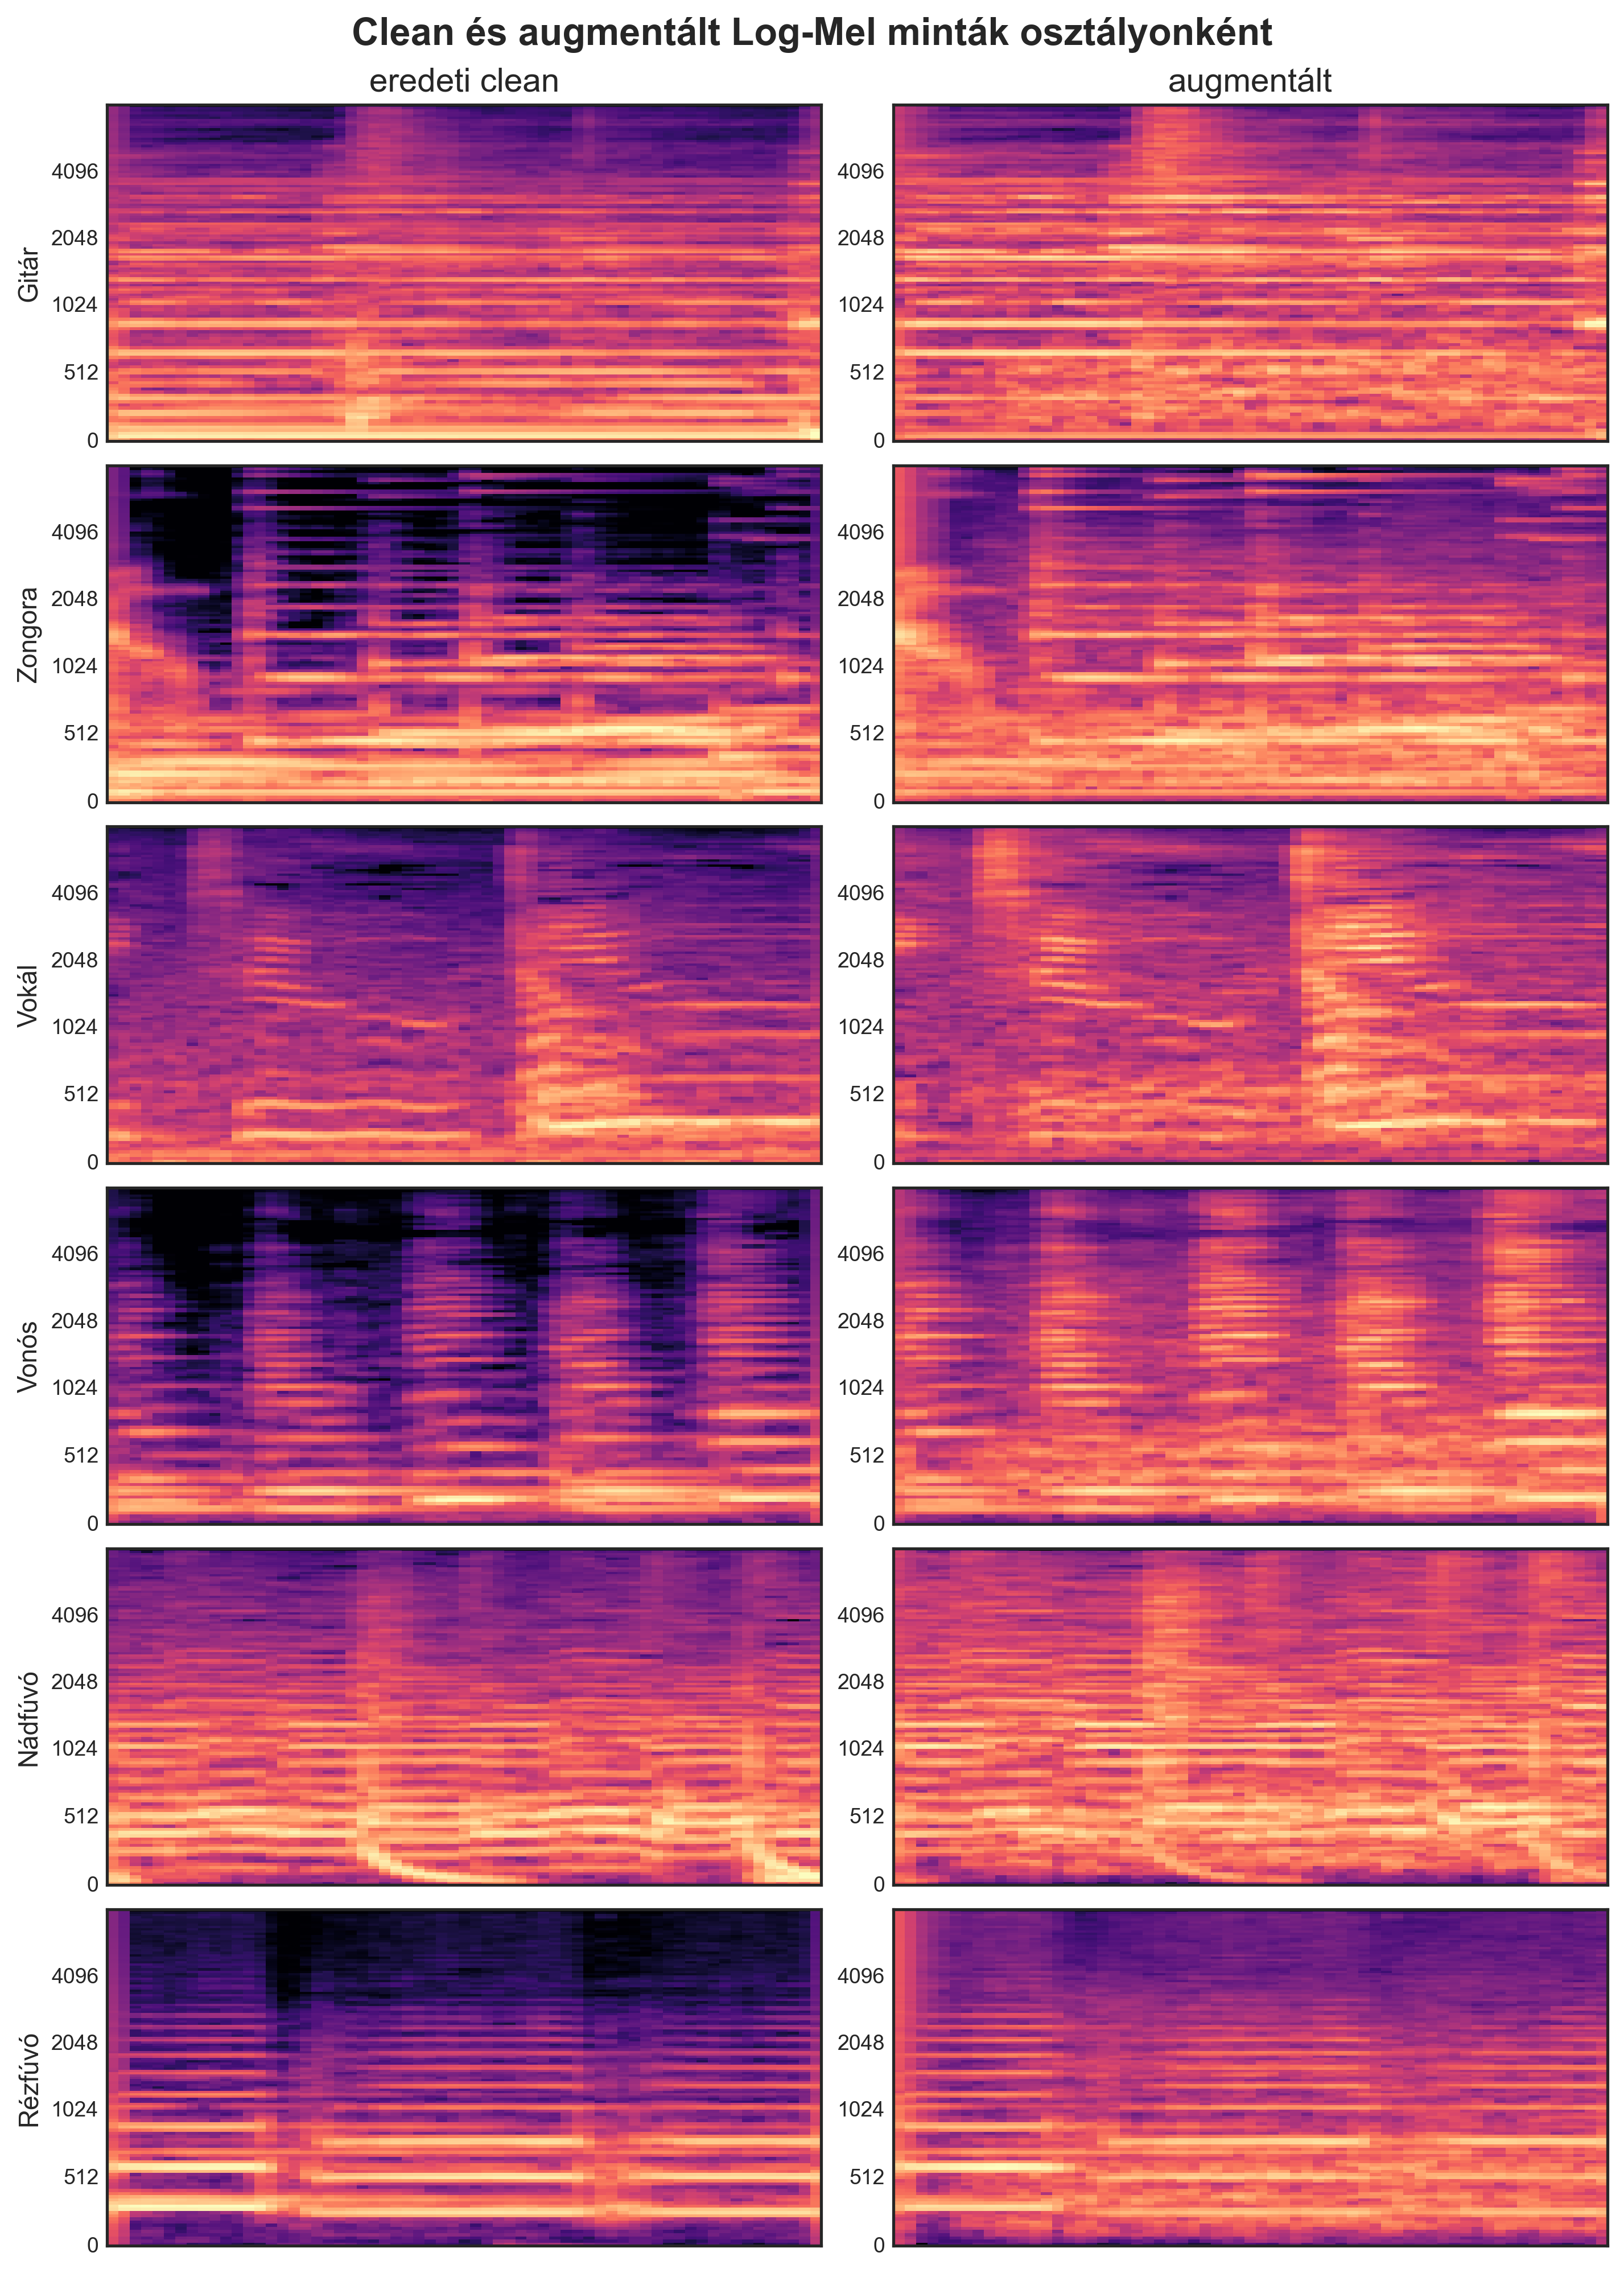
\includegraphics[height=0.74\textheight,keepaspectratio]{fig_original_vs_augmented.png}
  \caption{A hat hangszerosztály (gitár, zongora, vokál, hegedű, klarinét, kürt) egy-egy reprezentatív mintájának normalizált Log-Mel spektrogramja az eredeti (tiszta) és az adataugmentált (MacBook/mikrofon szimulációs lánccal torzított) állapotban}
  \label{fig:original_vs_augmented}
\end{figure}

Az augmentáció eredményeként a 6 hangszerosztály \textbf{tanító (train) halmazának tiszta mintái} kiegészülnek egy-egy torzított változattal (a \texttt{noise} és a már eleve mikrofonnal rögzített \texttt{\_mic\_} mintákat a script logikája automatikusan kihagyja).

Az augmentációs eljárás helyességének és minőségének manuális ellenőrzése, illetve összehasonlítása céljából a rendszer minden hangszerosztályból kiment néhány bemutató mintát (az eredeti és az augmentált változat párosait) az \texttt{augmented\_preview/} könyvtárba. Ez a gyakorlatban lehetővé teszi a fejlesztő számára, hogy mind füllel (hallás útján), mind vizuálisan meggyőződjön arról, hogy az alkalmazott szimulációs torzítások (például visszhang és zajkeverés) valósághűek, és nem teszik felismerhetetlenné a hangszerek alapvető karakterét.

%% ═══════════════════════════════════════════════════════════════════════════
\section{Modell architektúrák tervezése}
\label{sec:cnn_architecture}

A tervezett hangszerfelismerő rendszer magját egy mély konvolúciós neurális hálózat (CNN) alkotja, amely a Log-Mel spektrogramok 2D-s vizuális mintázatait tanulja meg osztályozni. Ebben a fejezetben részletezem a hálózat felépítését, a rétegek sorrendjét és paramétereit, valamint a hálózat betanításához használt konfigurációkat. A tervezett hálózati rétegek specifikációit a \ref{tab:cnn_standard}.~táblázat foglalja össze, a rétegek közötti adatfolyamot és az architektúra grafikus felépítését pedig a \ref{fig:cnn_architecture}.~ábra ábrázolja.

\subsection{A hálózati architektúra részletei}
\label{subsec:cnn_details}

A rendszer magját egy VGG-stílusú, háromblokkos konvolúciós hálózat (2D CNN) alkotja, kiegészítve egy bemeneti SpecAugment réteggel. A SpecAugment menet közben véletlenszerű idő- és frekvenciamaszkolással takar ki részleteket a spektrogramból, így kényszerítve a hálózatot az átfogóbb mintázatok megtanulására és a túlilleszkedés (overfitting) elkerülésére. A konvolúciós blokkok két egymást követő 2D konvolúcióból, Batch Normalization-ből, ReLU aktivációból, majd végül Max Poolingból és Dropoutból (30\%) állnak. A hálózat bemenete a kiválasztott, normalizált Log-Mel spektrogram ($64 \times 32 \times 1$), a kimenetnél pedig a hagyományos Flatten helyett térbeli átlagolást (GlobalAveragePooling2D) alkalmazunk a paraméterszám drasztikus csökkentése érdekében.

\begin{table}[H]
\centering
\caption{A tervezett 2D CNN architektúra rétegei (Log-Mel bemenet: $64 \times 32 \times 1$)}
\label{tab:cnn_standard}
\resizebox{\textwidth}{!}{
\begin{tabular}{llll}
\toprule
\textbf{Réteg} & \textbf{Szűrők / Neuronok} & \textbf{Kimenet} & \textbf{Paraméterek} \\
\midrule
SpecAugment & max 15 frekvencia, 8 idő maszk & $64 \times 32 \times 1$ & 0 \\
\midrule
2$\times$ Conv2D+BN+ReLU & 32 szűrő, $3 \times 3$, same & $64 \times 32 \times 32$ & $320 + 128 + 9\,248 + 128$ \\
MaxPool2D + Dropout & $2 \times 2$, dropout: 0{,}3 & $32 \times 16 \times 32$ & 0 \\
\midrule
2$\times$ Conv2D+BN+ReLU & 64 szűrő, $3 \times 3$, same & $32 \times 16 \times 64$ & $18\,496 + 256 + 36\,928 + 256$ \\
MaxPool2D + Dropout & $2 \times 2$, dropout: 0{,}3 & $16 \times 8 \times 64$ & 0 \\
\midrule
2$\times$ Conv2D+BN+ReLU & 128 szűrő, $3 \times 3$, same & $16 \times 8 \times 128$ & $73\,856 + 512 + 147\,584 + 512$ \\
GlobalAvgPool2D + Drop & dropout: 0{,}5 & 128 & 0 \\
\midrule
Dense + BN + ReLU & 128 neuron & 128 & $16\,512 + 512$ \\
Dropout & 0{,}5 & 128 & 0 \\
Dense & 7, Softmax & 7 & 903 \\
\midrule
\textbf{Összesen} & & & $\sim$306\,150 \\
\bottomrule
\end{tabular}
}
\end{table}

\begin{figure}[H]
\centering
\begin{tikzpicture}[
    node distance=0.8cm and 0.5cm,
    layer/.style={draw, rectangle, minimum height=0.8cm, minimum width=3.5cm, align=center, font=\footnotesize, rounded corners},
    input/.style={layer, fill=green!5!white, text width=4.5cm},
    block/.style={layer, fill=blue!5!white, text width=5.2cm, minimum height=1.3cm},
    dense/.style={layer, fill=orange!5!white, text width=5.2cm, minimum height=1.3cm},
    output/.style={layer, fill=red!5!white, text width=4.5cm},
    arrow/.style={thick,->,>=stealth}
]
  % Nodes
  \node (input) [input] {Bemenet \& SpecAugment \\ (Log-Mel: $64 \times 32 \times 1$)};
  
  \node (block1) [block, below=of input] {\textbf{1. Konvolúciós blokk} \\ 2x Conv2D (32 szűrő, $3\times3$, ReLU, BN) \\ MaxPool ($2\times2$) $\rightarrow$ Dropout (0,30) \\ \textit{Kimenet: $32 \times 16 \times 32$}};
  
  \node (block2) [block, below=of block1] {\textbf{2. Konvolúciós blokk} \\ 2x Conv2D (64 szűrő, $3\times3$, ReLU, BN) \\ MaxPool ($2\times2$) $\rightarrow$ Dropout (0,30) \\ \textit{Kimenet: $16 \times 8 \times 64$}};
  
  \node (block3) [block, below=of block2] {\textbf{3. Konvolúciós blokk} \\ 2x Conv2D (128 szűrő, $3\times3$, ReLU, BN) \\ GlobalAveragePooling2D $\rightarrow$ Dropout (0,50) \\ \textit{Kimenet: 128 dimenziós vektor}};
  
  \node (flatten) [dense, below=of block3] {\textbf{Közös fully connected rétegek} \\ Dense (128 neuron, ReLU) \\ BatchNorm $\rightarrow$ Dropout (0,50)};
  
  \node (output) [output, below=of flatten] {\textbf{Kimeneti réteg} \\ Dense (7 neuron, Softmax) \\ \textit{Hangszerosztály valószínűségek}};
  
  % Arrows
  \draw [arrow] (input) -- (block1);
  \draw [arrow] (block1) -- (block2);
  \draw [arrow] (block2) -- (block3);
  \draw [arrow] (block3) -- (flatten);
  \draw [arrow] (flatten) -- (output);
\end{tikzpicture}
\caption{A tervezett 2D CNN hálózati architektúra felépítése és adatfolyama}
\label{fig:cnn_architecture}
\end{figure}



\subsection{YAMNet Transfer Learning architektúra}
\label{subsec:yamnet_architecture}

Bár a saját fejlesztésű 2D CNN hálózat stabil teljesítményt nyújt (78\%-os baseline pontosság), a valós környezet sokrétű zajai és a felvételi torzítások kihívásai miatt szükség volt egy még stabilabb, jobban általánosító modellre. Ennek eléréséhez a Google által fejlesztett és a TensorFlow Hub-on publikált YAMNet modellt választottam ki. 

A YAMNet egy mély, MobileNetV1 alapú architektúra, amelyet a hatalmas AudioSet adatbázison tanítottak be, így kiváló akusztikai reprezentációs képességekkel rendelkezik. A YAMNet bemenete közvetlenül a normalizált nyers hanghullám ($16\,000$ elemű vektor).

A rendszeremben a YAMNet modellt nem a nulláról tanítom újra, hanem jellemzőkinyerőként (feature extractor) használom. A folyamat során az 1 másodperces audiojel végighalad a YAMNet befagyasztott konvolúciós rétegein, aminek az eredménye egy 1024 dimenziós sűrű reprezentáció (beágyazás, azaz \textit{embedding}). 

Ezt a mély beágyazást egy saját tervezésű, teljesen összekapcsolt (fully connected) osztályozó hálózatba vezetem be. Az általam tervezett osztályozó felépítése a következő:
\begin{enumerate}
  \item \textbf{Bemenet:} 1024 dimenziós YAMNet embedding
  \item \textbf{Rejtett réteg 1:} Sűrű réteg (Dense), 256 neuron, ReLU aktiváció
  \item \textbf{Normalizáció 1:} Batch Normalization és 40\% Dropout
  \item \textbf{Rejtett réteg 2:} Sűrű réteg (Dense), 128 neuron, ReLU aktiváció
  \item \textbf{Normalizáció 2:} Batch Normalization és 40\% Dropout
  \item \textbf{Kimeneti réteg:} Sűrű réteg (Dense), 7 neuron, Softmax aktiváció (hangszerosztályok valószínűségei)
\end{enumerate}

Ez az architektúra nemcsak, hogy drasztikus pontosságnövekedést (akár 90\% körüli F1-score) és sokkal stabilabb működést eredményezett a saját CNN baseline-hoz képest, de a tanítási időt is jelentősen lecsökkentette.

\subsection{Tanítási konfiguráció}


A 2D CNN modell tanítása során alkalmazott konfigurációt és hiperparamétereket úgy válogattam meg, hogy biztosítsák a modell stabil konvergenciáját és elkerüljék a túlilleszkedést (overfitting), miközben hatékonyan kihasználják a rendelkezésre álló számítási erőforrásokat. A modell optimalizálását, a veszteségfüggvényt, az adathalmaz felosztását és a tanulási folyamatot szabályozó callback mechanizmusokat a \ref{tab:training_config}.~táblázat foglalja össze részletesen.

\begin{table}[H]
\centering
\caption{A modell tanításához használt konfigurációs paraméterek és beállítások}
\label{tab:training_config}
\begin{tabular}{lp{8.0cm}}
\toprule
\textbf{Paraméter / Beállítás} & \textbf{Érték / Részletek} \\
\midrule
Optimalizáló & AdamW (tanulási ráta: $10^{-3}$, weight decay: $10^{-4}$) \\
Veszteségfüggvény & Categorical Crossentropy (Label Smoothing: 0,1 alkalmazásával) \\
Tanító/validációs/teszt & 70\% / 15\% / 15\% (rétegzett felosztásban) \\
Batch méret & 32 \\
Maximális epochszám & 150 \\
Early Stopping & \texttt{val\_loss} monitorozás, patience = 10, legjobb súlyok visszaállítása (\texttt{restore\_best\_weights=True}) \\
ReduceLROnPlateau & \texttt{val\_loss} monitorozás, patience = 4, faktor = 0{,}5, minimális tanulási ráta: $10^{-6}$ \\
ModelCheckpoint & \texttt{val\_accuracy} alapján a legjobb modell mentése \texttt{.keras} formátumban \\
\bottomrule
\end{tabular}
\end{table}

A táblázatban szereplő beállítások elméleti háttere és működési célja a következő:
\begin{itemize}
  \item \textbf{AdamW optimalizáló és Címkesimítás (Label Smoothing):} A hagyományos Adam helyett az AdamW optimalizálót (súlycsökkenés / weight decay bevonásával), a veszteségfüggvénynél pedig 0,1-es címkesimítást alkalmaztam. Ez a két technika együttesen erősen bünteti a modell túlzott magabiztosságát (overconfidence), ezáltal nagymértékben megelőzve a túlilleszkedést a zajos hangmintáknál.
  \item \textbf{Early Stopping callback:} Megakadályozza az iterációk felesleges futását. Ha a validációs veszteség (\texttt{val\_loss}) 10 egymást követő epochoz tartozóan már nem csökken, a tanítási folyamat automatikusan leáll, és visszaállítja a modellt a legjobb állapotba.
  \item \textbf{ReduceLROnPlateau callback:} Lehetővé teszi a tanulási ráta menet közbeni finomhangolását. Ha a modell elakad egy lokális minimum közelében (azaz a \texttt{val\_loss} nem csökken 4 epoch óta), a tanulási sebességet lefelezi ($0{,}5$-ös faktor), így segítve a precízebb konvergenciát.
\end{itemize}

A tanítás a Google Colab felhőszolgáltatás GPU-ján történik, az adatokat és a mentett modelleket a Google Drive-on tároljuk és onnan töltjük vissza a projektbe.

\subsubsection{A tanítás során generált kimenetek}
\label{subsubsec:model_outputs}

A tanítás lefutását követően a validációs adathalmazon legjobban teljesítő modellállapotok a projekt gyökerében lévő \texttt{models/} könyvtárba kerülnek mentésre. A különböző jellemzőtípusok alapján a következő fájlok jönnek létre:
\begin{itemize}
  \item \textbf{Log-Mel alapú CNN modell:} \texttt{best\_log\_mel\_2dcnn\_model.keras},
  \item \textbf{STFT alapú CNN modell:} \texttt{best\_stft\_2dcnn\_model.keras},
  \item \textbf{MFCC alapú CNN modell:} \texttt{best\_mfcc\_2dcnn\_model.keras}.
\end{itemize}
A TensorFlow \texttt{.keras} formátuma magában foglalja a hálózat architektúráját, a betanult súlymátrixokat, valamint az optimalizáló állapotát is. Ezen kimenetek közvetlenül betölthetőek a \texttt{tf.keras.models.load\_model} függvény segítségével, ami lehetővé teszi, hogy a valós idejű felismerő modul másodpercek alatt elinduljon a korábban elmentett legjobb modellállapot betöltésével.


%% ═══════════════════════════════════════════════════════════════════════════
\section{A valós idejű felismerő modul tervezése}
\label{sec:realtime}

A valós idejű hangszerfelismerő modul célja, hogy a számítógép mikrofonján keresztül érkező folyamatos audiojelet valós időben dolgozza fel, és minimális késleltetéssel jelezze ki a felismert hangszert és a predikció konfidenciaértékét. A modul stabil, aszinkron működésének megvalósításához egy többszálú architektúrát és egy egyedi predikciós stabilizáló logikát terveztem.

\subsection{Audio stream és aszinkron pufferelés}

A valós idejű hangfelvétel és a jelfeldolgozási lépések szétválasztásához többszálú jelfeldolgozó láncot alkalmazok. A hangkártya fizikai bemenetének kezeléséért a \texttt{sounddevice} könyvtár \texttt{InputStream} API-ja felel, amely egy magas prioritású háttérszálon futó hardveres megszakítási visszahívásos (callback) mechanizmusra épül:

\begin{itemize}
  \item \textbf{Mintavételi frekvencia ($f_s$):} 16\,000~Hz,
  \item \textbf{Csatornaszám:} 1 (monó),
  \item \textbf{Lépésköz (Step duration):} $0,25$ másodperc (4000 minta).
\end{itemize}

A beérkező audioadatok kezelése egy szálbiztos FIFO soron (\texttt{queue.Queue}) keresztül történik. Az audio callback függvény kizárólag a hardver pufferéből érkező 4000 mintás csomagokat helyezi el a sorban, majd azonnal visszatér. Ez garantálja, hogy a CPU-igényes neurális hálózati következtetés és a terminálfrissítés nem blokkolja a hangkártya illesztőprogramját, elkerülve az audió puffer alulcsordulását (buffer underflow).

A fő feldolgozó szál folyamatosan olvassa a sorból a 0,25 másodperces blokkokat. A predikció alapját egy folyamatos, $1,0$ másodperces (16\,000 minta) csúszóablak képezi. A 75\%-os átfedés (overlap) eléréséhez egy körpuffer-szerű logikát alkalmazok: minden új 0,25 másodperces blokk beérkezésekor a puffer tartalmát balra csúsztatom 4000 mintával, és az új adatot a puffer végére írom (roll művelet). Ezáltal a rendszer másodpercenként négyszer hajt végre predikciót az utolsó 1 másodpercnyi hanganyagra vonatkozóan.

\subsection{Jellemzőkinyerés és normalizálás}

A felismerő rendszer alapvetően kétféle hálózattal tud elindulni. Amennyiben a saját fejlesztésű 2D CNN hálózatot használjuk, minden predikciós ciklusban az 1 másodperces pufferből kinyerem a Log-Mel spektrogram jellemzőket. A kinyert spektrális mátrix dimenziója $128 \times 63$, ami megegyezik a tanítás során használt bemenettel.

A 2D CNN bemeneti rétege $[0, 1]$ intervallumba skálázott adatokat vár. A valós idejű jellemzőkre a tanítási fázissal azonos normalizálást alkalmazok decibel alapú korlátokkal:
$$X_{\text{norm}} = \frac{X_{\text{dB}} + 80,0}{80,0}$$
A kapott értékeket a $[0, 1]$ intervallumra vágom le (\texttt{clip} művelet), majd a tenzort átformázom a $1 \times 128 \times 63 \times 1$ bemeneti formára (batch és csatorna dimenziók hozzáadásával).

A fejlettebb, YAMNet alapú felismerő modul esetében az eljárás jóval egyszerűbb: a teljes, 16\,000 mintás nyers audiopuffert közvetlenül átalakítjuk TensorFlow tenzorrá, amiből a lefagyasztott YAMNet elkészíti az 1024-es beágyazást (embedding). Ezt az embedding vektort kapja meg a saját betanított osztályozónk.

\subsection{Zaj-alapú küszöbölés és Predikciós stabilizáció}

A hangszerosztályok pillanatnyi valószínűségei a zenefájlokban és az élő játékban tapasztalható dinamikus változások (tranziensek, vibrato, környezeti zajok) miatt gyorsan ingadozhatnak. Ha közvetlenül az aktuális predikció legnagyobb valószínűségű osztályát jelenítenénk meg, a terminálon zavaró, gyors váltások (,,villogás'') jelennének meg. Ennek kiszűrésére egy összetett stabilizációs logikát terveztem:

\begin{enumerate}
  \item \textbf{Temporális mozgóátlag simítás:} A modell kimeneti valószínűség-vektorait egy $W = 6$ elemű FIFO sorban tárolom (amely a 250 ms-os lépésköz miatt az utolsó $1,5$ másodperc predikciós történetét fedi le). A döntéshozatal a simított valószínűség-vektor alapján történik:
  $$\bar{p}_c^{(t)} = \frac{1}{W} \sum_{i=0}^{W-1} p_c^{(t-i)}$$
  
  \item \textbf{Hiszterézis mechanizmus:} Annak érdekében, hogy megakadályozzuk a két közeli valószínűségű osztály közötti ugrálást (chattering), egy $H = 0,05$ ($5\%$) értékű hiszterézis bónuszt adunk a jelenleg aktív (kijelzett) osztály $C^{(t-1)}$ simított valószínűségéhez a maximumkeresés előtt:
  $$a_c^{(t)} = \bar{p}_c^{(t)} + H \cdot \mathbb{I}(c = C^{(t-1)})$$
  ahol $\mathbb{I}$ az indikátorfüggvény. A jelölt új osztályt a módosított vektor maximumhelye adja meg.
  
  \item \textbf{Osztály-specifikus konfidencia-küszöb:} Nem alkalmazok fix hardveres RMS alapú zajkaput, mivel a modell kiválóan megtanulta a \texttt{noise} (zaj/csend) osztály felismerését. Helyette a predikció során osztály-specifikus küszöbértékeket ellenőrzök, amelyek értékeit az alábbi empirikus megfontolások alapján határoztam meg:
  \begin{itemize}
      \item \textbf{Hangszerek küszöbe ($45\%$):} Mivel 7 kategóriánk van, egy teljesen véletlenszerű döntés $\sim$14\%-os valószínűséget jelentene. A 45\%-os küszöb megköveteli, hogy a modell határozottan dominánsnak ítélje meg a felismert hangszert. Ezzel elkerülhetők a vakriasztások (false positives), amik a zajosabb tranziensek vagy műfajok közötti átmenetek során 20-30\%-os tüskeként jelentkezhetnének.
      \item \textbf{Zaj/Csend küszöbe ($20\%$):} Amikor a hangszeres játék befejeződik, a mikrofonba csak a szoba alapzaja jut. Ilyenkor a neurális hálózat gyakran bizonytalanabb, és a kimeneti valószínűséget szétkeni a többi 6 osztály között, így a \texttt{noise} kimenet ritkán éri el a 45\%-ot. Ha a zajhoz is magas küszöböt követelnénk, a kijelző "beleragadna" az utolsó hangszer állapotába. A mindössze 20\%-os (de még mindig az egyenletes eloszlásnál magasabb) küszöb biztosítja, hogy a rendszer agresszívan és gyorsan visszaálljon az alapállapotra (csendre), amint a hangszer elhalkul.
  \end{itemize}
  A kijelzett hangszercsere tehát csak akkor történik meg, ha a vizsgált osztály simított valószínűsége átlépi a rá vonatkozó küszöböt. Ez a szoftveres megoldás feleslegessé teszi a jelszint alapú RMS számítást.
\end{enumerate}

Ez a tervezési megoldás rendkívül stabil vizuális visszajelzést biztosít a felhasználói felületen, miközben a gyorsabb, 0,25 másodperces frissítési ütemnek köszönhetően a rendszer rendkívül reszponzív marad. A valós idejű felismerési folyamat egyes lépéseit a \ref{fig:realtime_pipeline}.~ábra foglalja össze vizuálisan.

\begin{figure}[H]
\centering
\begin{tikzpicture}[
    node distance=0.8cm and 1.0cm,
    flowblock/.style={draw, rectangle, minimum height=1.0cm, minimum width=3.0cm, fill=blue!5!white, align=center, font=\footnotesize, rounded corners, text width=2.9cm},
    flowio/.style={draw, rectangle, minimum height=1.0cm, minimum width=3.0cm, fill=green!5!white, align=center, font=\footnotesize, rounded corners, text width=2.9cm},
    flowproc/.style={draw, rectangle, minimum height=1.0cm, minimum width=3.0cm, fill=orange!5!white, align=center, font=\footnotesize, rounded corners, text width=2.9cm},
    flowout/.style={draw, rectangle, minimum height=1.0cm, minimum width=3.0cm, fill=red!5!white, align=center, font=\footnotesize, rounded corners, text width=2.9cm},
    flowarrow/.style={thick,->,>=stealth}
]
  % Nodes
  \node (mic) [flowio] {Mikrofon \\ (élő audio stream)};
  \node (seg) [flowblock, right=of mic] {Csúszóablak \\ (1 másodperc, 16\,000 minta)};
  \node (mel) [flowproc, right=of seg] {Log-Mel jellemzők \\ (128 $\times$ 63 mátrix)};
  \node (norm) [flowproc, right=of mel] {Normalizálás \\ ($[0,1]$ skálázás)};
  
  \node (cnn) [flowblock, below=of norm] {2D CNN predikció \\ (osztály valószínűségek)};
  \node (avg) [flowproc, left=of cnn] {Mozgóátlag simítás \\ ($W=6$ puffer, hiszterézis)};
  \node (disp) [flowout, left=of avg] {Kijelzés \\ (hangszer + konfidencia)};
  
  % Arrows
  \draw [flowarrow] (mic) -- (seg);
  \draw [flowarrow] (seg) -- (mel);
  \draw [flowarrow] (mel) -- (norm);
  \draw [flowarrow] (norm) -- (cnn);
  \draw [flowarrow] (cnn) -- (avg);
  \draw [flowarrow] (avg) -- (disp);
\end{tikzpicture}
\caption{A valós idejű felismerési folyamat lépései az élő hangbeviteltől a kijelzésig}
\label{fig:realtime_pipeline}
\end{figure}

%% ═══════════════════════════════════════════════════════════════════════════
\section{A feldolgozási folyamat összefoglaló áttekintése}
\label{sec:pipeline_overview}

A teljes rendszer a tervezéstől a megvalósításig egymásra épülő fázisokból áll, amelyek a teljes adatfeldolgozási és tanítási láncot lefedik. Ezeket a tervezési fázisokat az alábbi számozott pontokban foglalom össze, a fázisok közötti összefüggéseket és a teljes rendszerfolyamatot pedig a \ref{fig:full_pipeline}.~ábra szemlélteti.

\begin{enumerate}
  \item \textbf{Tiszta adathalmaz előkészítése} (\texttt{01\_prepare\_clean\_dataset.py}): A forrásfájlok Train/Val/Test rétegzett elosztása csoportszinten (leakage elkerülése), majd 1 másodperces szeletelés.
  \item \textbf{Mikrofonos újrafelvétel} (\texttt{02\_acquire\_mic\_data.py}): A tiszta tanító halmaz kimentése, folyamatos audióvá fűzése, majd telefonos lejátszás közbeni mikrofonos rögzítése és újraszeletelése.
  \item \textbf{Adathalmazok fúziója és ellenőrzése} (\texttt{03a\_merge\_mic\_to\_train.py} és \texttt{03b\_check...}): A mikrofonos minták beolvasztása kizárólag a tanító (train) halmazba, majd a darabszámok integritásvizsgálata.
  \item \textbf{Jellemzőkinyerés és augmentáció} (\texttt{04a\_extract\_features.py}): Log-Mel, STFT, MFCC mátrixok és nyers hullámformák kinyerése, kiegészítve a tiszta train minták szoftveres torzításával (reverb, zajkeverés, pre-emphasis).
  \item \textbf{Modell tanítása} (\texttt{06\_train\_model\_colab/} mappában): A saját 2D CNN (VGG-stílusú) és a YAMNet Transfer Learning modellek betanítása Google Colab GPU-n.
  \item \textbf{Valós idejű felismerés} (\texttt{05a\_realtime\_...} vagy \texttt{05b\_realtime\_yamnet.py}): Élő, mikrofonos hangbevitel valós idejű feldolgozása, jellemzőkinyerése és stabilizált predikciója (0,25 másodpercenként).
\end{enumerate}

\begin{figure}[H]
\centering
\begin{tikzpicture}[
    node distance=0.6cm,
    flowstep/.style={draw, rectangle, minimum height=0.9cm, minimum width=9.5cm, fill=blue!5!white, align=left, font=\footnotesize, rounded corners, text width=9.3cm},
    arrow/.style={thick,->,>=stealth}
]
  % Nodes
  \node (s1) [flowstep] {\textbf{1. Tiszta adathalmaz előkészítése} (\texttt{01\_prepare\_clean\_dataset.py}) \\ Rétegzett elosztás (Train/Val/Test) a leakage elkerülésével, majd 1mp-es szeletelés};
  
  \node (s2) [flowstep, below=of s1] {\textbf{2. Mikrofonos újrafelvétel} (\texttt{02\_acquire\_mic\_data.py}) \\ A train halmaz folyamatos lejátszása, mikrofonos rögzítése és újraszeletelése};
  
  \node (s3) [flowstep, below=of s2] {\textbf{3. Adathalmazok fúziója} (\texttt{03a\_merge\_...}, \texttt{03b\_check\_...}) \\ Mikrofonos minták beolvasztása a train halmazba, integritás ellenőrzése};
  
  \node (s4) [flowstep, below=of s3] {\textbf{4. Jellemzőkinyerés \& Augmentáció} (\texttt{04a\_extract\_...}, \texttt{04b\_check\_...}) \\ Spektrogramok/nyers jel kinyerése + train minták szoftveres torzítása $\rightarrow$ \texttt{.npy}};
  
  \node (s5) [flowstep, below=of s4] {\textbf{5. Modell tanítása} (\texttt{06\_train\_model\_colab} scriptek) \\ CNN és YAMNet modellek betanítása Colab GPU-n (AdamW, Label Smoothing)};
  
  \node (s6) [flowstep, below=of s5] {\textbf{6. Valós idejű felismerés} (\texttt{05a\_realtime\_...} / \texttt{05b\_...}) \\ Élő audio stream feldolgozása, predikciós simítás és kijelzés};

  % Arrows
  \draw [arrow] (s1) -- (s2);
  \draw [arrow] (s2) -- (s3);
  \draw [arrow] (s3) -- (s4);
  \draw [arrow] (s4) -- (s5);
  \draw [arrow] (s5) -- (s6);
\end{tikzpicture}
\caption{A hangszerfelismerő rendszer végső adatfeldolgozási és tanítási folyamatának lépései}
\label{fig:full_pipeline}
\end{figure}
